\begin{lstlisting}
p15 16 17(3)(4)(8)(9)(10)
p38 3(3)(5) 4 5 6 8 10    
\end{lstlisting}
\begin{figure}[H]
\centering
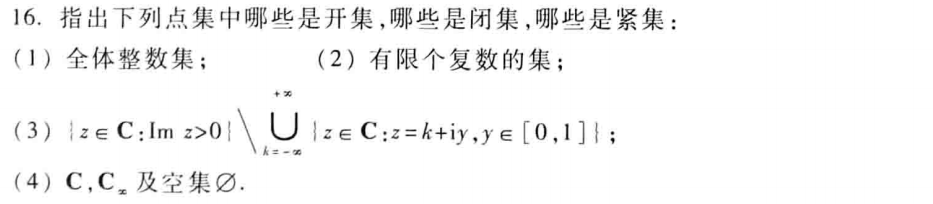
\includegraphics[width=\textwidth]{hw2-20250318.png}
% \caption{}
\label{}
\end{figure}

在复平面拓扑下:

(1) $\mathbb{Z}$ 不含内点,故不是开集,$\mathbb{Z}$ 没有聚点,故为闭集。由于 $\mathbb{C}$ 同构于 $\mathbb{R}^{2}$ ,故 $E\subset \mathbb{C}$ 是紧集当且仅当 $E$ 是有界闭集,但 $\mathbb{Z}$ 并非有界,故 $\mathbb{Z}$ 不是紧集。

(2) 同理于 (1),该集合不是开集,是闭集,是紧集。

(3) 令
\[
E=\{ z\in \mathbb{C} :\mathrm{Im}z>0\}\setminus \bigcup_{k=-\infty}^{+\infty} \{ z\in \mathbb{C}:z=k+iy,y\in[0,1] \}
\]
\begin{figure}[H]
\centering
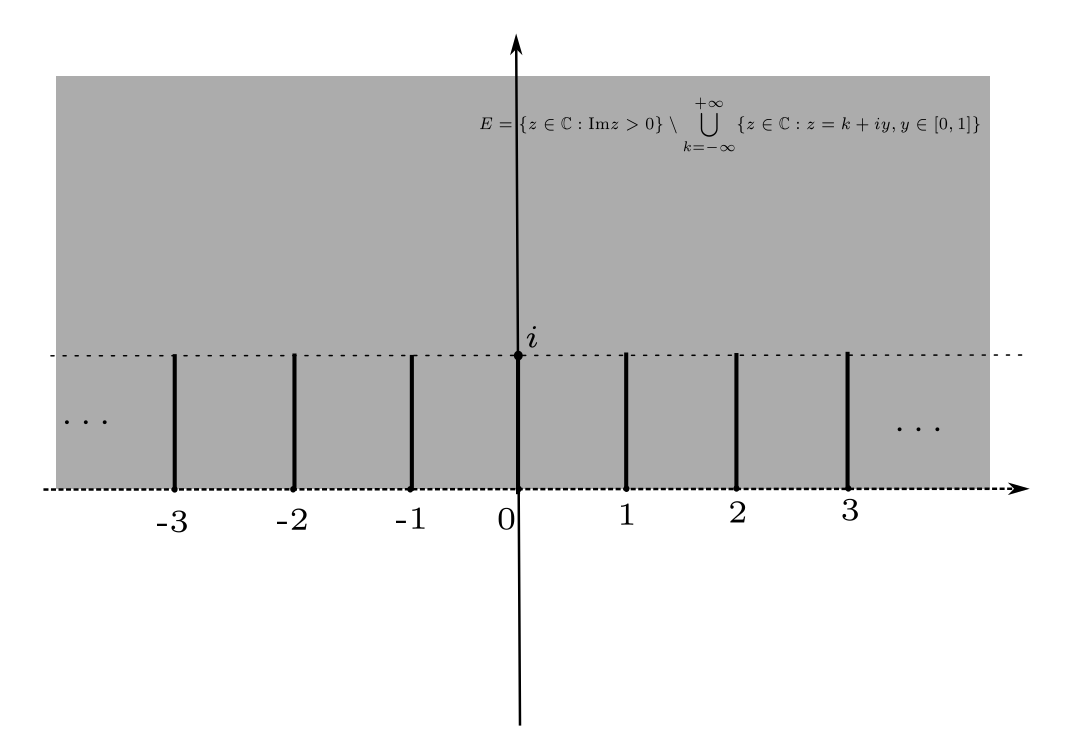
\includegraphics[width=\textwidth]{1-hw2-20250318.png}
% \caption{}
\label{}
\end{figure}

所有点都是内点,所以 $E$ 是开集。而任意 $z=k+iy, k\in \mathbb{Z}, y\in[0,1]$ 作为极限点,却不在 $E$ 中,故 $E$ 不是闭集,进而不是紧集。

(4) 显然 $\mathbb{C}$ 是开集,不是闭集,不是紧集。$\mathbb{C}_{\infty}$ 是闭集,是开集,是紧集。$\varnothing$ 是开集,是闭集,是紧集。

\begin{remark}
$\mathbb{C}_{\infty}$ 的定义是黎曼球球极投影得到的,它是依照 $\mathbb{R}^{3}$ 中的 $S^2$ 表面拓扑而定的。它是 $\mathbb{C}$ 的紧致化。
\end{remark}
\begin{figure}[H]
\centering
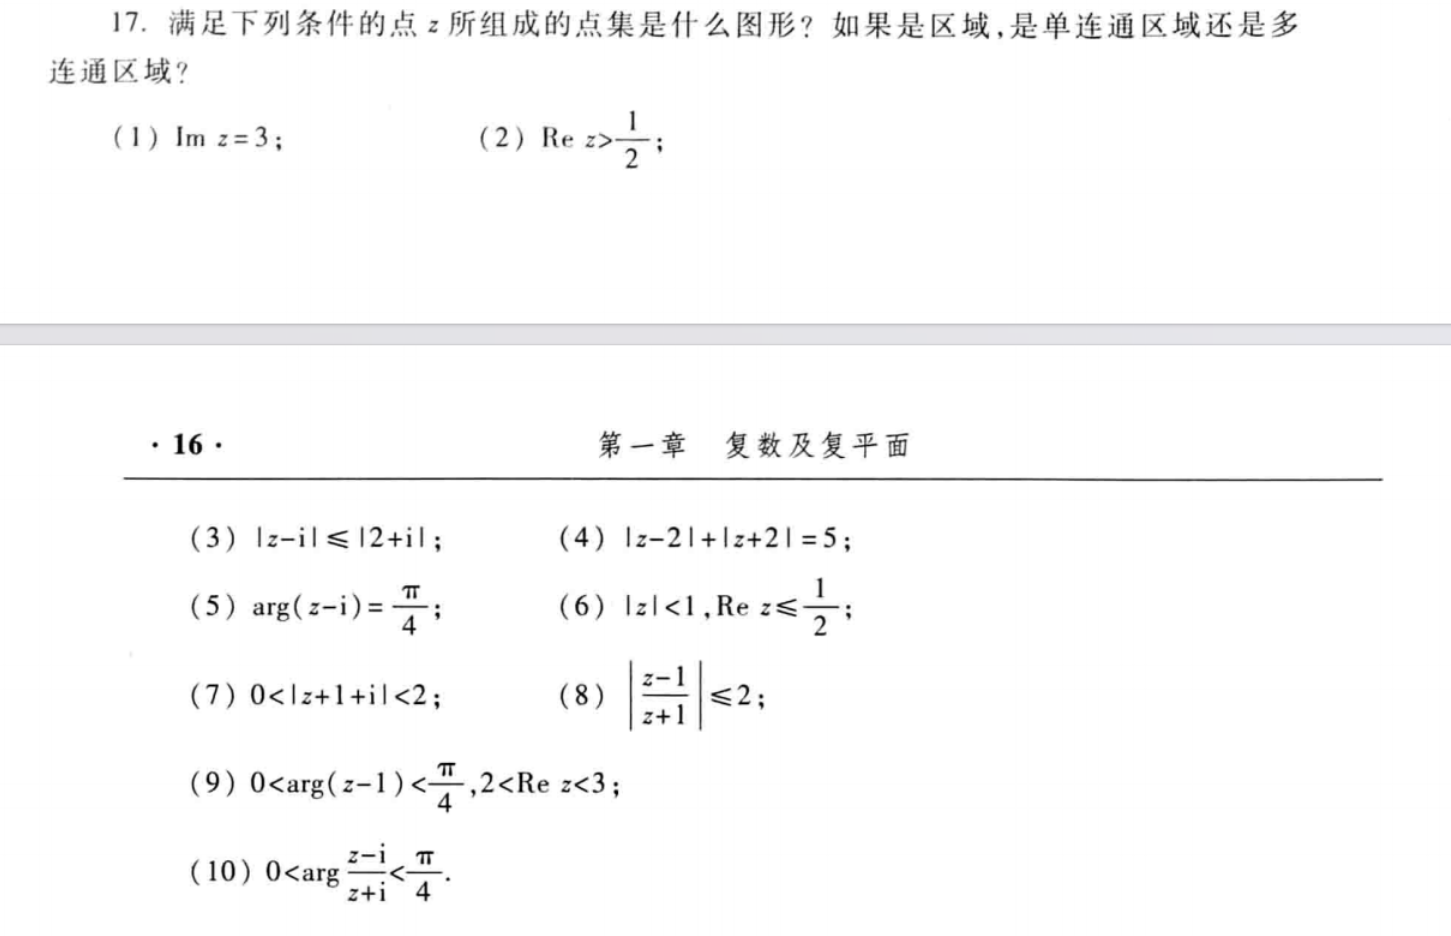
\includegraphics[width=\textwidth]{2-hw2-20250318.png}
% \caption{}
\label{}
\end{figure}

(3)
\begin{figure}[H]
\centering
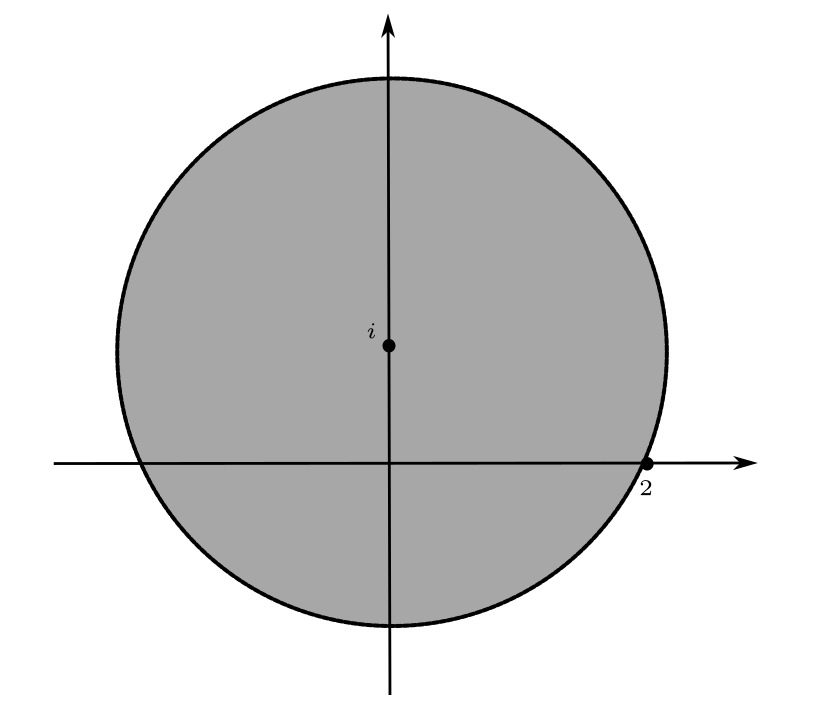
\includegraphics[width=\textwidth]{3-hw2-20250318.png}
% \caption{}
\label{}
\end{figure}
单连通的闭圆盘

(4)
\[
\lvert z-2 \rvert +\lvert z+2 \rvert =5
\]
设 $z=x+iy$,那么
\[
\sqrt{ (x-2)^{2}+y^{2} }+\sqrt{ (x+2)^{2}+y^{2} }=5
\]
平方得到
\[
(x-2)^{2}+y^{2}=(5-\sqrt{ (x+2)^{2}+y^{2} })^{2}=25+(x+2)^{2}+y^{2}-10\sqrt{ (x+2)^{2}+y^{2} }
\]
化简得到
\[
10\sqrt{ (x+2)^{2}+y^{2} }=25+8x
\]
平方得到
\[
100(x+2)^{2}+100y^{2}=625+400x+64x^{2}
\]
化简得到
\[
36x^{2}+100y^{2}=625
\]
是一个椭圆,显然单连通。

(8)
\[
\left|\frac{z-1}{z+1}\right| \leqslant 2 
\]
设 $z=x+iy$,则
\[
\sqrt{ (x+1)^{2}+y^{2} }\neq 0,\quad \sqrt{ (x-1)^{2}+y^{2} }\leq 2\sqrt{ (x+1)^{2}+y^{2} }
\]
于是 $(x,y)\neq(-1,0)$. 平方得到
\[
x^{2}-2x+1+y^{2}\leq4x^{2}+8x+4+4y^{2}
\]
化简得到
\[
3x^{2}+10x+3y^{2}+3\geq 0
\]
也就是说
\[
\left( x^{2}+\frac{10}{3}x+\frac{25}{9} \right)+y^{2}\geq \frac{16}{9}
\]
即
\[
\left( x+\frac{5}{3} \right)^{2}+y^{2}\geq  \frac{16}{9}\text{ 且 }(x,y)\neq (-1,0)
\]
这是复平面挖掉一个圆盘,显然单连通。
\begin{figure}[H]
\centering
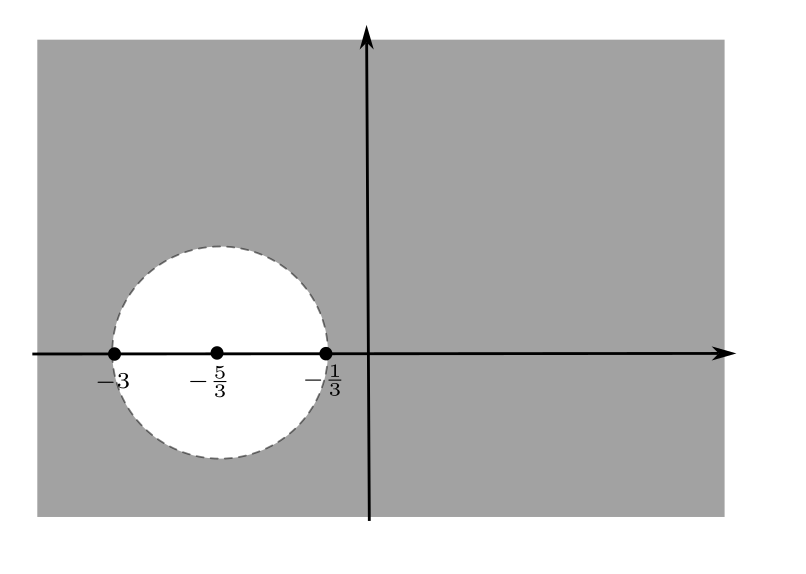
\includegraphics[width=\textwidth]{7-hw2-20250318.png}
% \caption{}
\label{}
\end{figure}

(9)
\[
0<\arg (z-1)<\frac{\pi}{4}, 2<\operatorname{Re} z<3
\]
\begin{figure}[H]
\centering
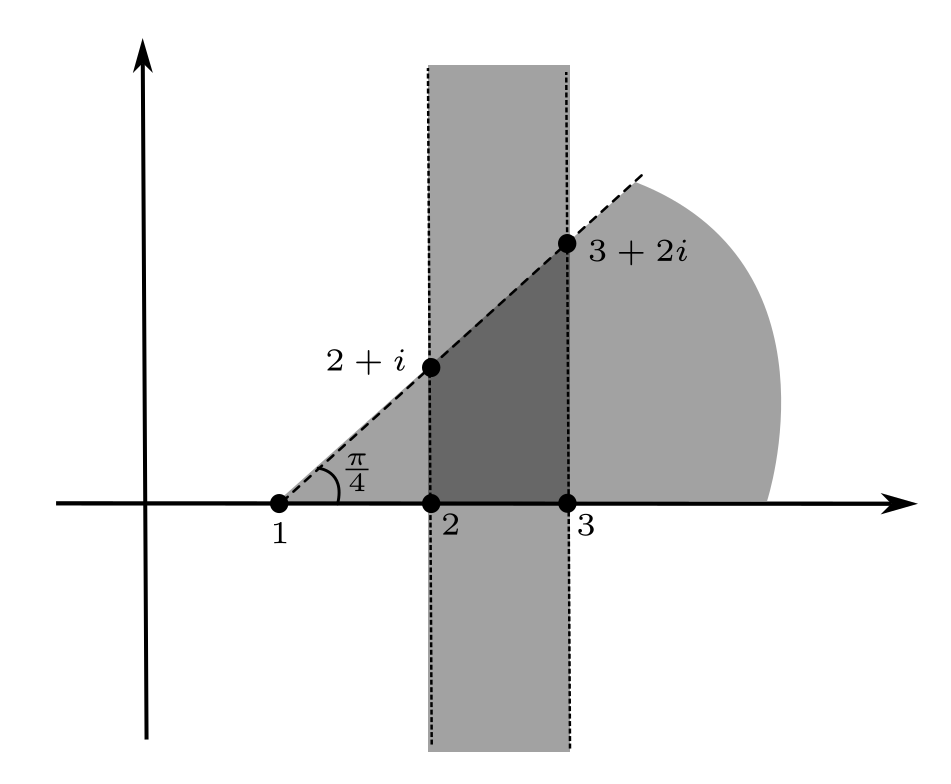
\includegraphics[width=\textwidth]{4-hw2-20250318.png}
% \caption{}
\label{}
\end{figure}

这是单连通区域

(10)
\[
0<\arg \frac{z-\mathrm{i}}{z+\mathrm{i}}<\frac{\pi}{4}
\]
设 $z=x+iy$,则
\[
\frac{z-i}{z+i}=\frac{x+i(y-1)}{x+i(y+1)}=\frac{(x+i(y-1))(x-i(y+1))}{x^{2}+(y+1)^{2}}=\frac{x^{2}+y^{2}-1-2xi}{x^{2}+(y+1)^{2}}
\]
于是,对于 $x=0$,$\arg\frac{z-i}{z+i}=0$,对于 $x\neq0$,则
\[
\arg\frac{z-i}{z+i}=\arctan\frac{x^{2}+y^{2}-1}{-2x}\in\left( 0,\frac{\pi}{4} \right)\Rightarrow\frac{x^{2}+y^{2}-1}{-2x}\in(0,1)
\]
若 $x>0$,则
\[
-2x<x^{2}+y^{2}-1<0
\]
也就是说
\[
x^{2}+y^{2}<1\text{ 且 }(x+1)^{2}+y^{2}>2
\]
\begin{figure}[H]
\centering
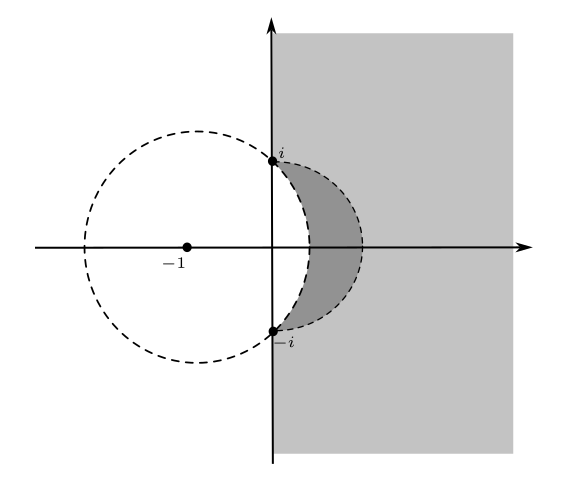
\includegraphics[width=\textwidth]{9-hw2-20250318.png}
% \caption{}
\label{}
\end{figure}

若 $x<0$,则
\[
0<x^{2}+y^{2}-1<-2x
\]
也就是说
\[
x^{2}+y^{2}>1\text{ 且 }(x+1)^{2}+y^{2}<2
\]
\begin{figure}[H]
\centering
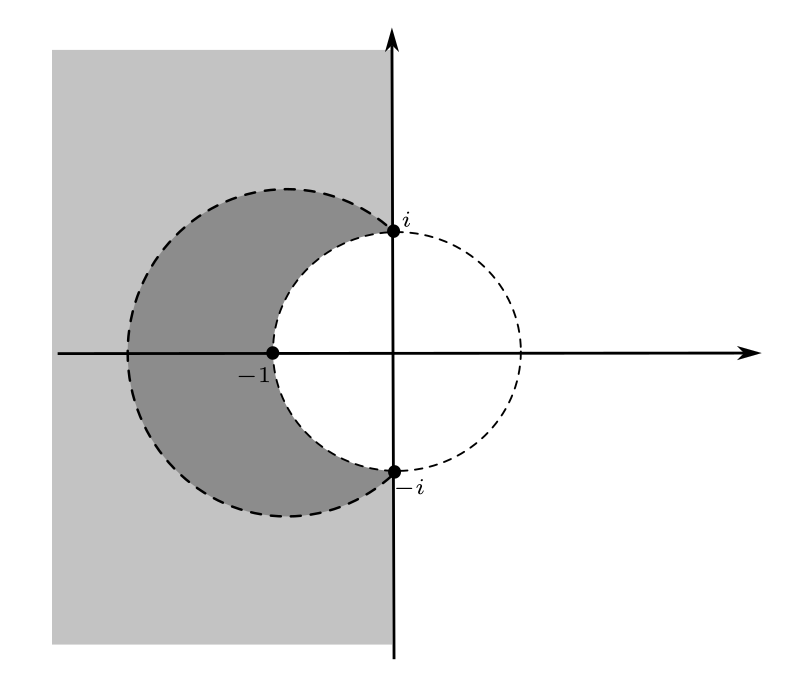
\includegraphics[width=\textwidth]{10-hw2-20250318.png}
% \caption{}
\label{}
\end{figure}

总而言之,该区域为

\begin{figure}[H]
\centering
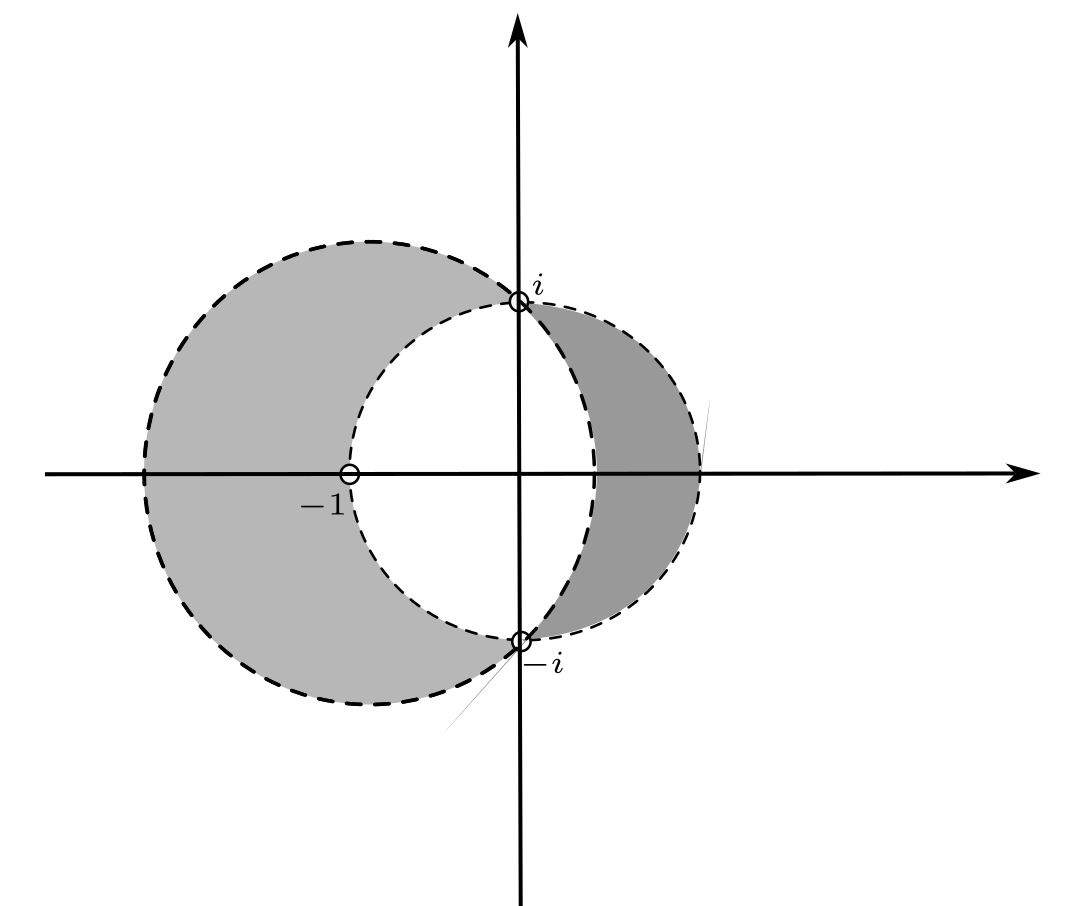
\includegraphics[width=\textwidth]{12-hw2-20250318.png}
% \caption{}
\label{}
\end{figure}

是多连通的开区域

\begin{figure}[H]
\centering
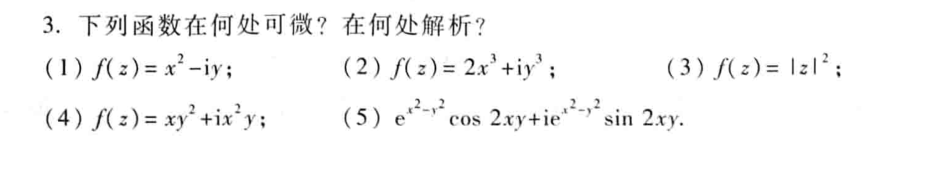
\includegraphics[width=\textwidth]{hw2-20250306.png}
% \caption{}
\label{}
\end{figure}

\begin{definition}[解析函数]
\begin{figure}[H]
\centering
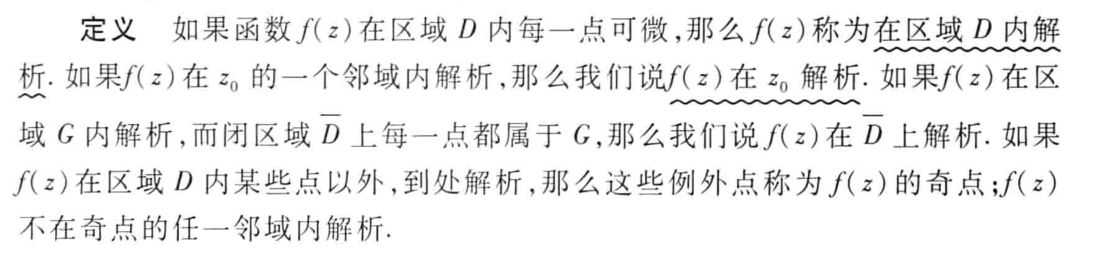
\includegraphics[width=\textwidth]{3-hw2-20250306.png}
% \caption{}
\label{}
\end{figure}
\end{definition}
\begin{theorem}
\begin{figure}[H]
\centering
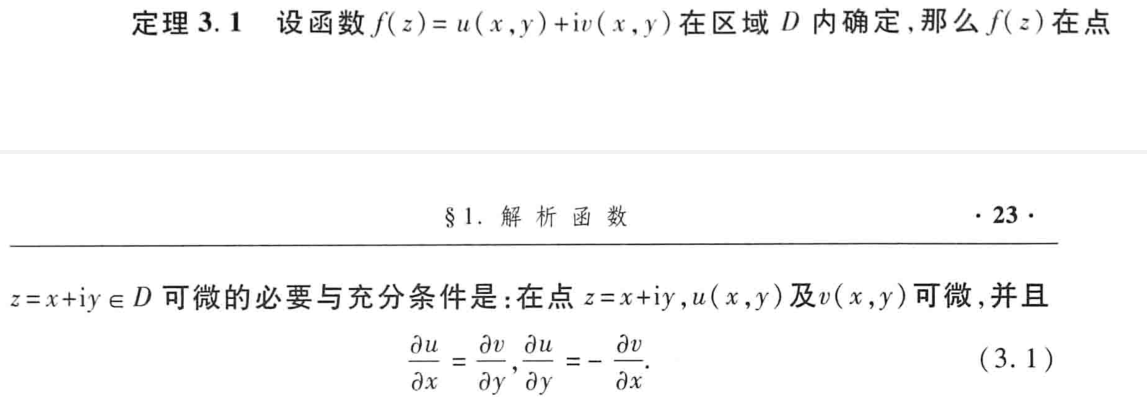
\includegraphics[width=\textwidth]{1-hw2-20250306.png}
% \caption{}
\label{}
\end{figure}
\end{theorem}
\begin{theorem}
\begin{figure}[H]
\centering
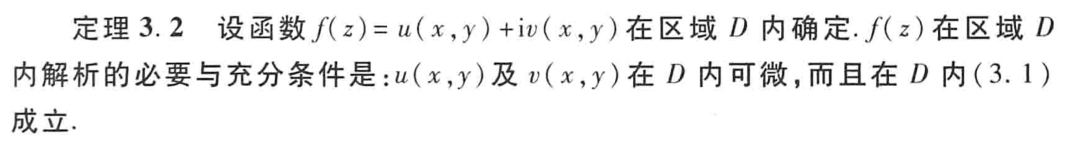
\includegraphics[width=\textwidth]{2-hw2-20250306.png}
% \caption{}
\label{}
\end{figure}
\end{theorem}
(3) $f (z)=x^{2}+y^{2}\eqqcolon u (x, y)+i v(x,y)$ so $u_{x}=2x,u_{y}=2y,v_{x}=v_{y}=0$. If $f(z)=\lvert z \rvert ^{2}$ is differentiable at $z_0=x_0+iy_0$ then $u_{x}=v_{y},u_{y}=-v_{x}$ implies that $x_0=y_0=0$ thus $z_0=0$. Hence $\,0$ is the only point at which $f$ is differentiable. For any neighborhood $U$ of $\,0$, $f$ is not differentiable in $U\setminus \{ 0 \}$ thus $f$ is not holomorphic over $U$. Therefore $f$ is holomorphic at no point.
(5) $f (z)=e^{ x^{2}-y^{2} }\cos (2xy)+ie^{ x^{2}-y^{2} }\sin (2xy)\eqqcolon u (x, y)+i v(x,y)$ so $u_{x}=2x\cos(2xy)e^{ x^{2}-y^{2} }-2y\sin(2xy)e^{ x^{2}-y^{2} }=v_{y}$, and $u_{y}=-2y\cos(2xy)e^{ x^{2}-y^{2} }-2x\sin(2xy)e^{ x^{2}-y^{2} }=-v_{x}$.

\begin{figure}[H]
\centering
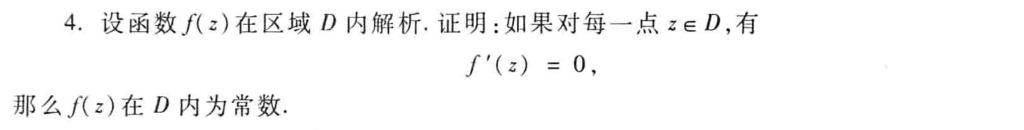
\includegraphics[width=\textwidth]{4-hw2-20250306.png}
% \caption{}
\label{}
\end{figure}

$f (z)\coloneqq u (x, y)+i v(x,y)$ for $z=x+iy$, since $f\in H(D)$ then $\overline{\partial}f (z)=0, z\in D$ where $\overline{\partial}\coloneqq \frac{1}{2}(\partial _{x}+i\partial_{y})$, and $\partial f (z)=f' (z)=0, z\in D$ where $\partial\coloneqq \frac{1}{2}(\partial_{x}-i \partial_{y})$, we have $\partial_{x}f=0,\partial_{y}f=0$, i.e. $u_{x}=v_{x}=0,u_{y}=v_{y}=0$. (the differentiability is derived from $f\in H(D)$ and theorem 3.2) Therefore $u\equiv c_1,v\equiv c_2$ constant, and $f\equiv u+iv=c_1+c_2$ is constant in $D$.

\begin{figure}[H]
\centering
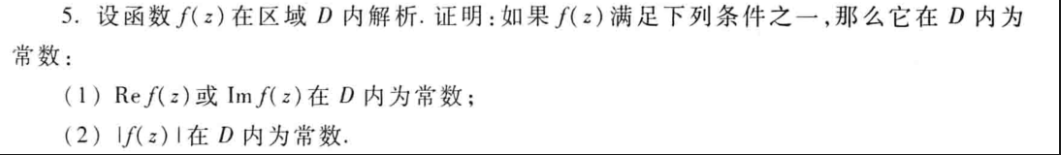
\includegraphics[width=\textwidth]{hw2-20250307.png}
% \caption{}
\label{}
\end{figure}

(1) $f (z)\coloneqq u(x,y)+i v(x,y)$ for $z=x+iy$. $f\in H(D)$ means $u, v\in H(D)$ and $\overline{\partial}f (z)=0, z\in D$, i.e. $\frac{1}{2}(\partial _{x}f(z)+i\partial_{y}f(z))=\frac{1}{2}(\partial_{x}u+i\partial_{x}v+i\partial_{y}u-\partial_{y}v)=0$. If $u=\mathrm{Re}f$ is constant in $D$ then $\partial_{x}u=\partial_{y}u=0$, combined with the fact that $\partial_{x}u-\partial_{y}v=0$ and $\partial_{x}v+\partial_{y}u=0$, we have $\partial_{x}u=\partial_{y}u=\partial_{x}v=\partial_{y}v=0$. Therefore $f$ is constant in $D$. There is a similar proof for $\mathrm{Im}f\equiv Const.$ in $D$.
(2) If $\lvert f \rvert\equiv c$  is a constant in $D$ then $\bar{f}=\frac{c^{2}}{f}$ is holomorphic in $D$. However, if both $u+i v$ and $u-i v$ satisfies the C-R equation, it is easy to get $u_{x}=u_{y}=v_{x}=v_{y}=0$ and thus $f$ is constant.

\begin{figure}[H]
\centering
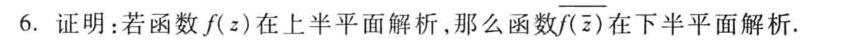
\includegraphics[width=\textwidth]{6-hw2-20250306.png}
% \caption{}
\label{}
\end{figure}

$f(z)\coloneqq u(x,y)+iv(x,y)$ for $z=x+i y$. $g(z)\coloneqq\overline{f (\overline{z})}=u (x,-y)-i v(x,-y)$. By theorem 3.2 it suffices to show that $u(x,-y)$ and $v(x,-y)$ are differentiable in $\mathbb{R}^{2}_{-}$ and $\overline{\partial}g(z)=0$ for $(x,y)\in \mathbb{R}^{2}_{-}$. By theorem 3.2 we have $u(x,y),v(x,y)$ are differentiable in $\mathbb{R}^{2}_{+}$ and $\overline{\partial}f(z)=0$, i.e. $\partial_{x}u=\partial_{y}v,\partial_{x}v=-\partial_{y}u$.
\[
\begin{aligned}
\overline{\partial }g(z) & =\frac{1}{2}(\partial _{x}+i\partial _{y})(u(x,-y)+i v(x,-y)) \\
 & =\frac{1}{2}\partial _{x}u(x,-y)-\frac{1}{2}i\partial _{x}v(x,-y)+\frac{1}{2}i\partial _{y}u(x,-y)-\frac{1}{2} \partial _{y}u(x,-y) \\
 & =\frac{1}{2}(u_{x}+v_{y})(x,-y)+\frac{1}{2}i(u_{y}-v_{x})(x,-y)=0\qquad \text{where }(x,-y)\in \mathbb{R}^{2}_{+}
\end{aligned}
\]
Therefore $\overline{f(\overline{z})}$ is holomorphic in the lower half plane.

\begin{figure}[H]
\centering
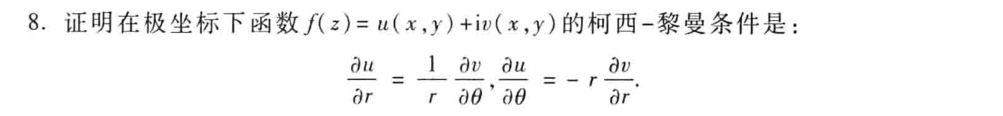
\includegraphics[width=\textwidth]{7-hw2-20250306.png}
% \caption{}
\label{}
\end{figure}

$x=r\cos\theta,y=r\sin\theta$. So we have
\[
\begin{aligned} 
\frac{ \partial u }{ \partial r }  & =\frac{ \partial u }{ \partial x }\frac{ \partial x }{ \partial r }+\frac{ \partial u }{ \partial y }\frac{ \partial y }{ \partial r } =\frac{ \partial u }{ \partial x } \cos\theta+\frac{ \partial u }{ \partial y } \sin\theta  \\
\frac{ \partial v }{ \partial r }  & =\frac{ \partial v }{ \partial x }\frac{ \partial x }{ \partial r }+\frac{ \partial v }{ \partial y }\frac{ \partial y }{ \partial r }=\frac{ \partial v }{ \partial x } \cos\theta+\frac{ \partial v }{ \partial y } \sin\theta \\
\frac{ \partial u }{ \partial \theta }  & =\frac{ \partial u }{ \partial x } \frac{ \partial x }{ \partial \theta } +\frac{ \partial v }{ \partial y } \frac{ \partial y }{ \partial \theta } =\frac{ \partial u }{ \partial x } (-r\sin\theta)+\frac{ \partial u }{ \partial y } r\cos\theta \\
\frac{ \partial v }{ \partial \theta }  & =\frac{ \partial v }{ \partial x } \frac{ \partial x }{ \partial \theta } +\frac{ \partial v }{ \partial y } \frac{ \partial y }{ \partial \theta } =\frac{ \partial v }{ \partial x } (-r\sin\theta)+\frac{ \partial v }{ \partial y } r\cos\theta
\end{aligned}
\]
Then
\[
\frac{ \partial u }{ \partial r } =\frac{1}{r}\frac{ \partial v }{ \partial \theta } \iff u_{x}r\cos\theta+u_{y}r\sin\theta=-v_{x}r\sin\theta+v_{y}r\cos\theta \iff(u_{x}-v_{y})x=-(v_{x}+u_{y})y
\]
And
\[
\frac{ \partial u }{ \partial \theta } =-r\frac{ \partial v }{ \partial r } \iff-u_{x}r\sin\theta+u_{y}r\cos\theta=-v_{x}r\cos\theta-v_{y}r\sin\theta \iff(u_{x}-v_{y})y=(u_{y}+v_{x})x
\]
The Cauchy-Riemann condition is $u_{x}=v_{y},u_{y}+v_{x}=0$, which means
\[
u_{r}\cdot \frac{ \partial r }{ \partial x } +u_{\theta}\cdot \frac{ \partial \theta }{ \partial x } =v_{r}\cdot \frac{ \partial r }{ \partial y }+v_{\theta}\cdot \frac{ \partial \theta }{ \partial y }\text{ and }u_{r}\cdot \frac{ \partial r }{ \partial y } +u_{\theta}\cdot \frac{ \partial \theta }{ \partial y } +v_{r}\cdot \frac{ \partial r }{ \partial x }+v_{\theta}\cdot \frac{ \partial \theta }{ \partial x }=0
\]
where $r=\sqrt{ x^{2}+y^{2} },\theta=\arctan \frac{y}{x}$ then
\[
\frac{ \partial r }{ \partial x }=\frac{x}{\sqrt{ x^{2}+y^{2} }}=\frac{x}{r},\frac{ \partial r }{ \partial y }=\frac{y}{\sqrt{ x^{2}+y^{2} }}=\frac{y}{r},\frac{ \partial \theta }{ \partial x } =-\frac{y}{x^{2}+y^{2}}=-\frac{y}{r^{2}} ,\frac{ \partial \theta }{ \partial y } =\frac{x}{x^{2}+y^{2}}=\frac{x}{r^{2}} 
\]
Therefore
\[
u_{r}\frac{x}{r}-u_{\theta}\frac{y}{x^{2}} =v_{r}\frac{y}{r}+v_{\theta}\frac{x}{r^{2}}\text{ and }u_{r}\frac{y}{r}+u_{\theta}\frac{x}{r^{2}}+v_{r}\frac{x}{r}-v_{\theta}\frac{y}{r^{2}}=0
\]
Hence
\[
\frac{ \partial u }{ \partial r } =\frac{1}{r}\frac{ \partial v }{ \partial \theta } ,\quad \frac{ \partial u }{ \partial \theta } =-r\frac{ \partial v }{ \partial r }
\]
\begin{figure}[H]
\centering
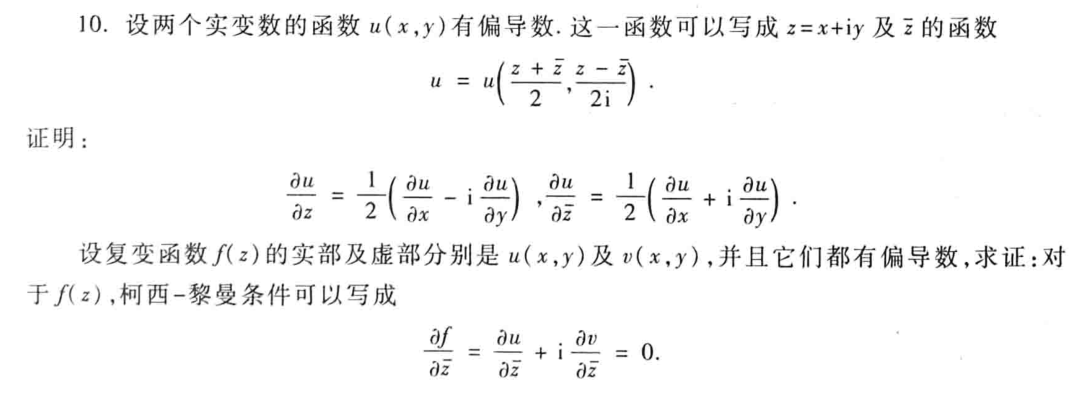
\includegraphics[width=\textwidth]{8-hw2-20250306.png}
% \caption{}
\label{}
\end{figure}
\[
\frac{ \partial u }{ \partial z } =\frac{ \partial u\left( \frac{z+\overline{z}}{2},\frac{z-\overline{z}}{2i} \right) }{ \partial z }=\frac{1}{2}\left( \frac{ \partial u }{ \partial x } -i\frac{ \partial u }{ \partial y }  \right),\quad \frac{ \partial u }{ \partial \bar{z} } =\frac{ \partial u\left( \frac{z+\overline{z}}{2},\frac{z-\overline{z}}{2i} \right) }{ \partial \bar{z} }=\frac{1}{2}\left( \frac{ \partial u }{ \partial x } +i\frac{ \partial u }{ \partial y }  \right)
\]
\[
\frac{ \partial f }{ \partial \bar{z} }=\frac{ \partial u }{ \partial \bar{z} } +i \frac{ \partial v }{ \partial \bar{z} } =\frac{1}{2}(u_{x}+iu_{y})+\frac{1}{2}i(v_{x}+iv_{y})=\frac{1}{2}(u_{x}-v_{y})+\frac{1}{2}i(u_{y}+v_{x})=0\iff u_{x}=v_{y},u_{y}=-v_{x}
\]
which is Cauchy-Riemann equation.
